\section{Design}

Develop repository design and basic trust approach for offline report generation and online real-time viewing of the data as typically used by Fac Mgmt. 

\paragraph{Challenges}
\begin{itemize}
\item Namespace design to tackle overlapping roles of names in application data access, routing, device deployment, security, etc. 
\item Storage/repository design that provides familiar query interfaces.
\item Discovery and bootstrapping that is easier and more secure than IP. 
\item Trust model development and implementation (a good problem to have). 
\item Efficient crypto performance and group / multi-cast cryptographic challenges. 
\item Low-frequency, high-importance notifications (alarms).
\end{itemize}

\paragraph{Approach.}

\begin{itemize}
\item A hierarchical namespace for sensor data, devices, and users that embodies intrinsic relationships in BMS applications and can be used directly for data delivery;
\item Bootstrapping and ongoing management of device configuration that is simpler, more scalable and more robust than IP solutions;
\item Per-packet signatures, applied immediately after data acquisition, that enable  straightforward verification of data authenticity and provenance;
\item Strong security through cryptographic signing to verify data authenticity and provenance;
\item Encryption-based access control to sensor data, with data encrypted immediately after its acquisition, rather than relying on encrypted channels; 
\item Strong privacy through encryption-based access control to protect sensing data, without reliance on physical/logical network isolation.
\item Identity-based authentication using NDN's (still developing) security primitives; 
\item Scalable user and privilege management to support enterprise-wide deployments. 
\end{itemize}




\subsection{NDN-EBAMS Application Architecture} 
 
\begin{figure}[!ht]
\centering
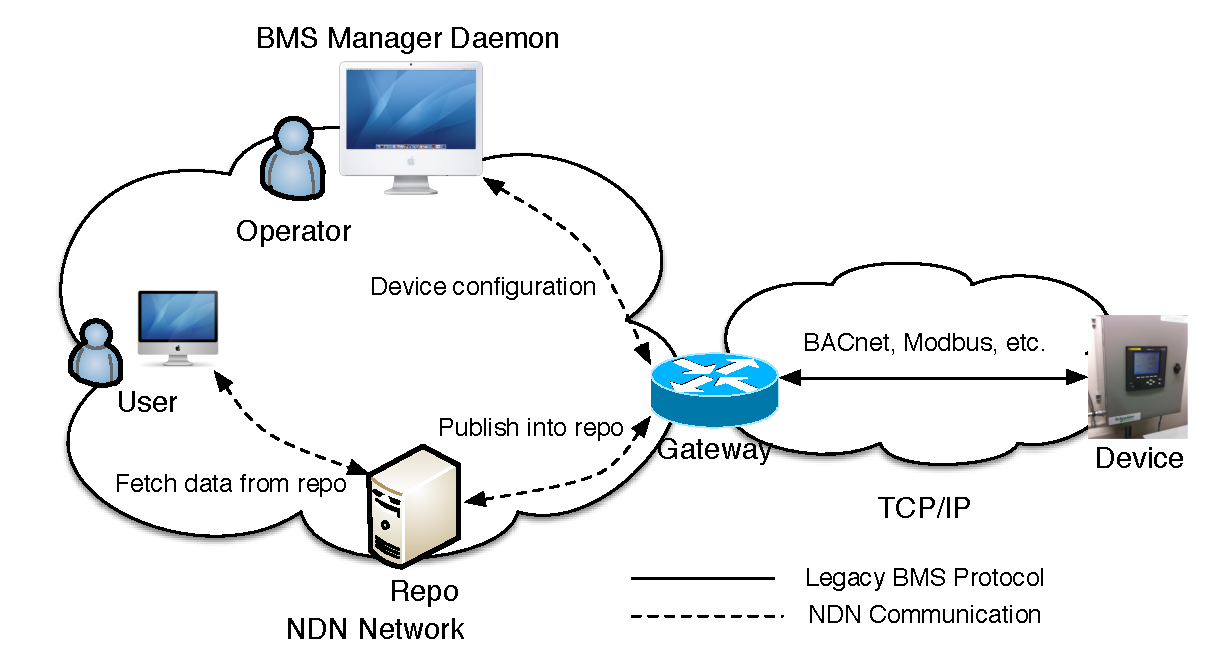
\includegraphics[width=0.7\textwidth, keepaspectratio=true]{figures/bms-arch.pdf}
\caption{Major components in NDN-EBAMS, where there are potentially many users and gateways, and multiple devices per gateway.}
\label{design:arch}
\end{figure}
 
Figure~\ref{design:arch} shows the initial design of NDN-EBAMS with three main entities: end users, sensor gateway (including the connected devices) and a privileged manager application controlled by human operators who handle out-of-band user authentication and privilege authorization. The manager application is responsible for gateway/device and user management over the NDN network.


Gateways insert sensor data into NDN Repositories (repos), which respond to user Interests for data in the sensor namespace. This indirection decouples data generation from user fetching and provides benefits of automatic data archiving, 
non-interactive access control (described below), and protection from DOS/DDOS attack on gateways. In our initial implementation, a Web interface fetches the data from the repo by issuing Interest packets with proper data prefixes.

A detailed description of the initial architecture can be found at~\cite{secure-ndn-bms-ieee}.

  
\subsection{Trust and security}
 
Only focus on read access control. No write access.

Opportunity to compare active services (e.g., broker) with passive. 

\subsubsection{Identity}

In NDN parlance, the concept of ``identity'' refers to the public key owned by some entity (which could be a device, a person, or an organization).
Since the keys and certificates are also published as NDN data packets on the network, each identity will receive a unique NDN name.
The human-readable and hierarchical identity name can express a rich set of trust relationships and makes it easier to specify the trust policies compared to using self-certifying hashes or public key bits.

\subsubsection{Trust model}

The hierarchical structure in the real-world facility management department forms a natural hierarchy of trust, similar to traditional Public Key Infrastructure (PKI).
In a typical deployment of EBAMS, there is a single root of trust owned by the manager of the entire enterprise.
The root manager may delegate responsibilities to lower-level managers who have control over a specific department or building by signing their identities.
The identity of the devices are signed by either the direct managers or other identities further delegated from the managers (such as the identity of a room or device rack).


\subsubsection{Integrity}

Each NDN data packet is signed by the publisher's identity.
The cryptographic signature provides a strong integrity protection.

\subsubsection{Confidentiality}

Given the nature of EBAMS, data confidentiality is often an essential requirement.
In NDN-EBAMS, confidentiality and access control is achieved through data encryption and controlling the distribution of the encryption key.
The EBAMS data may be accessed by a large number of users with different types of privileges.
For example, enterprise employees may have limited access to the data according to the place they work in or the department they belong to, while the utility companies may have external access to only a certain type of data (such as electricity) across the entire campus.
The challenge is to design a efficient and flexible key distribution scheme that can scale to a large number of users and satisfy the diversified privilege requirements.

Should we mention the idea of APL/ACL here?

% Groups: NDN-BmS developers at UCLA, UIUC, departmental/campus stakeholders, and testbed users. 
% Users:  Users possessing a cert in new system, and anonymous users on the web.
% Applications that are not associated with a real-world users but need credentials: aggregators, gateways, background processes, etc. 

% There appear to be two important factors to
% consider in controlling access to a specific monitoring point or group of
% points in our pilot: 1) what department it relates to (not necessarily in the name),
% 2) what type of data it is (probably in the name).
% Each "point" here corresponds to a source of time-series monitoring data.
% For UCLA, I would expect there are O(100) "departments", with many
% individuals having access for several departments, and O(10) types of
% data, for our purposes.

% What is the appropriate practical crypto scheme to develop access control
% based on these dimensions?  I really like the concept of ABE, as long as
% there is some ability to deploy it practically, because it would enable us
% to define sensible *named* attributes that correspond directly to
% department and data type. A relationship between attribute names and data
% names (for key data, etc.) might be useful to simplify things at the
% application level.



\subsection{Naming}
\subsubsection{Data}


In BMS protocols such as BACnet, it is common to name devices to reflect their physical location.
We follow this convention for data naming in NDN-BMS and constructs the namespace based on the hierarchy in the building structure.   
For example, the building (identified by its real-world name or label) may be (optionally) partitioned into \emph{floors} (identified by the floor number) first, and then by \emph{rooms} (identified by the room number). 
Devices may be further grouped by the physical attachment (e.g., different panels) and/or the functionality (e.g., power, voltage, temperature, etc.). Critically, the namespace schema for a given BMS can, to a large extent, remain at the discretion of those who install and manage the system. For example, in our prototype we name \textit{data} rather than the \textit{devices} that collect it, but could use devices names instead or in addition. 

Similarly, operators can choose the scope or granularity of responsibility for a given gateway.
In the example of Figure~\ref{design:ns}, we have one gateway that covers the entire Strathmore building, while another gateway is only responsible for a single studio in Melnitz Hall.
Finer granularity reduces the load of a single gateway device but can increase management complexity.
Note that it is straightforward to configure a gateway to publish in a certain part of the hierarchy - it just registers the appropriate prefix with its upstream hub, a process that is out of scope for this paper but a straightforward part of the architecture, and then publishes data under that prefix. 

\begin{figure}[!ht]
\centering
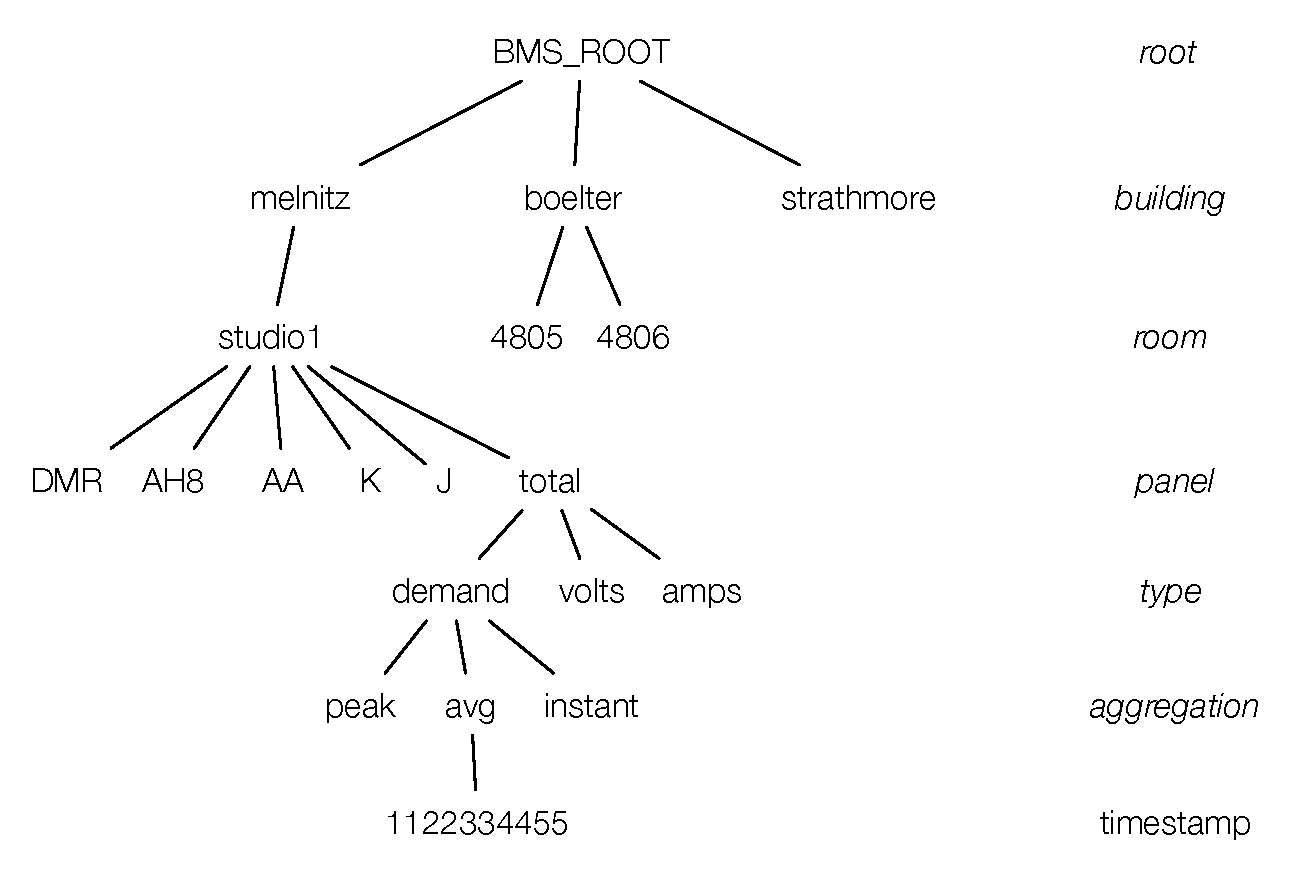
\includegraphics[width=0.8\textwidth, keepaspectratio=true]{figures/bms-namespace-new.pdf}
\caption{Example NDN-BMS namespace design for the prototype deployment at UCLA.}
\label{design:ns}
\end{figure}

Figure~\ref{design:ns} shows the NDN-BMS namespace used by the UCLA campus testbed.
The root node represents the common prefix for UCLA BMS namespace (\url{/ndn/ucla.edu/bms}).
The NDN name of a sensor data packets (e.g., \url{/ndn/ucla.edu/bms/building/melnitz/studio/1/data/panel/J/voltage/<timestamp>} in Figure~\ref{design:ns}) indicates the physical location of the sensor (Panel J inside Studio 1, Melnitz Hall), the type of data (voltage) and the time when the data is acquired, expressed as a timestamp in the last component of the name.
If the data packet contains aggregated data (i.e., a series of data points generated within a given time window), the timestamp reflects the generation time of the first data point in the series. 
The timestamp-based versioning allows BMS users to fetch sensor data within any time range once the data is archived in the repo.

% Discover
% Design focuses on the actual deployment
% Data sources \& sinks:  sensors, actuators.
% Physical space / location will be involved in trust and should be described consistently and considered along with routing / application implications.
% Approach to naming/retrieving sample batches. 
% Approach to metadata describing sensor feeds. 

% Hierarchical data names and simple sensor/control abstraction.
See also: 

Dawson-Haggerty, Stephen, et al. "Enabling green building applications." Proceedings of the 6th Workshop on Hot Topics in Embedded Networked Sensors. ACM, 2010.

Ortiz, Jorge, and David Culler. A system for managing physical data in buildings. Technical Report No. EECS-2010-128, EECS Department, University of California, Berkeley, 2010.

Potentially can use names for:
\begin{itemize}
\item Abstraction (allow application generalization)
\item Organization (by building area, system topology) 
\item Metadata access (consistent approach)
\item Aggregation (hierarchy inferred from names) 
\end{itemize} 



BOSS~\cite{Dawson-Haggerty2013BOSS} follows these references for building metadata. 

[8] Bazjanac, V., et al. HVAC component data modeling using industry foundation classes. In System Simulation in Buildings (2002). 

[30] Liu, X. et al, Requirements for a formal approach to represent information exchange requirements of a self-managing framework for HVAC systems. In ICCCBE (2012). 

[40] Project Haystack. http://project-haystack.org/  


\subsubsection{Certificates}

\subsection{Storage}

Repository for time-series data used in BOSS~\cite{Dawson-Haggerty2013BOSS} is readingdb, \url{https://github.com/stevedh/readingdb}.
%% TODO: Review BOSS paper and incorporate here. 
Their simplification of repositories is about data type more than query type:  focus on time series data from points. 
MySQL not used because of expensive insert and poor scaling with large number of leaf keys.
Low latency application interface for accessing the large repository of data at different granularity, a selection language, and a data transformation language. Enabling the construction of a pipeline of operators to the retrieved data. 

Repository requirements to support sql-style access

Designing and deploying hierarchical repositories for sensor data (from sensor module to panel to building to campus scale) that provide quick access to fresh data and efficient, redundant long-term storage. 

More activity on repo-ng needed? 

Reasonable performance on a variety of device classes  running as a component in a data producer and as a centralizer of data. 

Write performance for main repo:  20,000 samples @ 1Hz on an ongoing basis.  

Mechanism to export / move data offline. 

Need a simple way to watch time-series prefixes. 

Restore sync support for more complex namespaces. 

\subsection{Routing \& Forwarding}

Limit packets inside and outside? 

\subsection{Communication}
Alarms
Efficient support for specific types of communication patterns found in these networks, like reliable notification of rare but critical events. 


\subsection{User Interface}
\subsubsection{Website}
